\begin{wrapfigure}{l}{0pt}
  \centering
  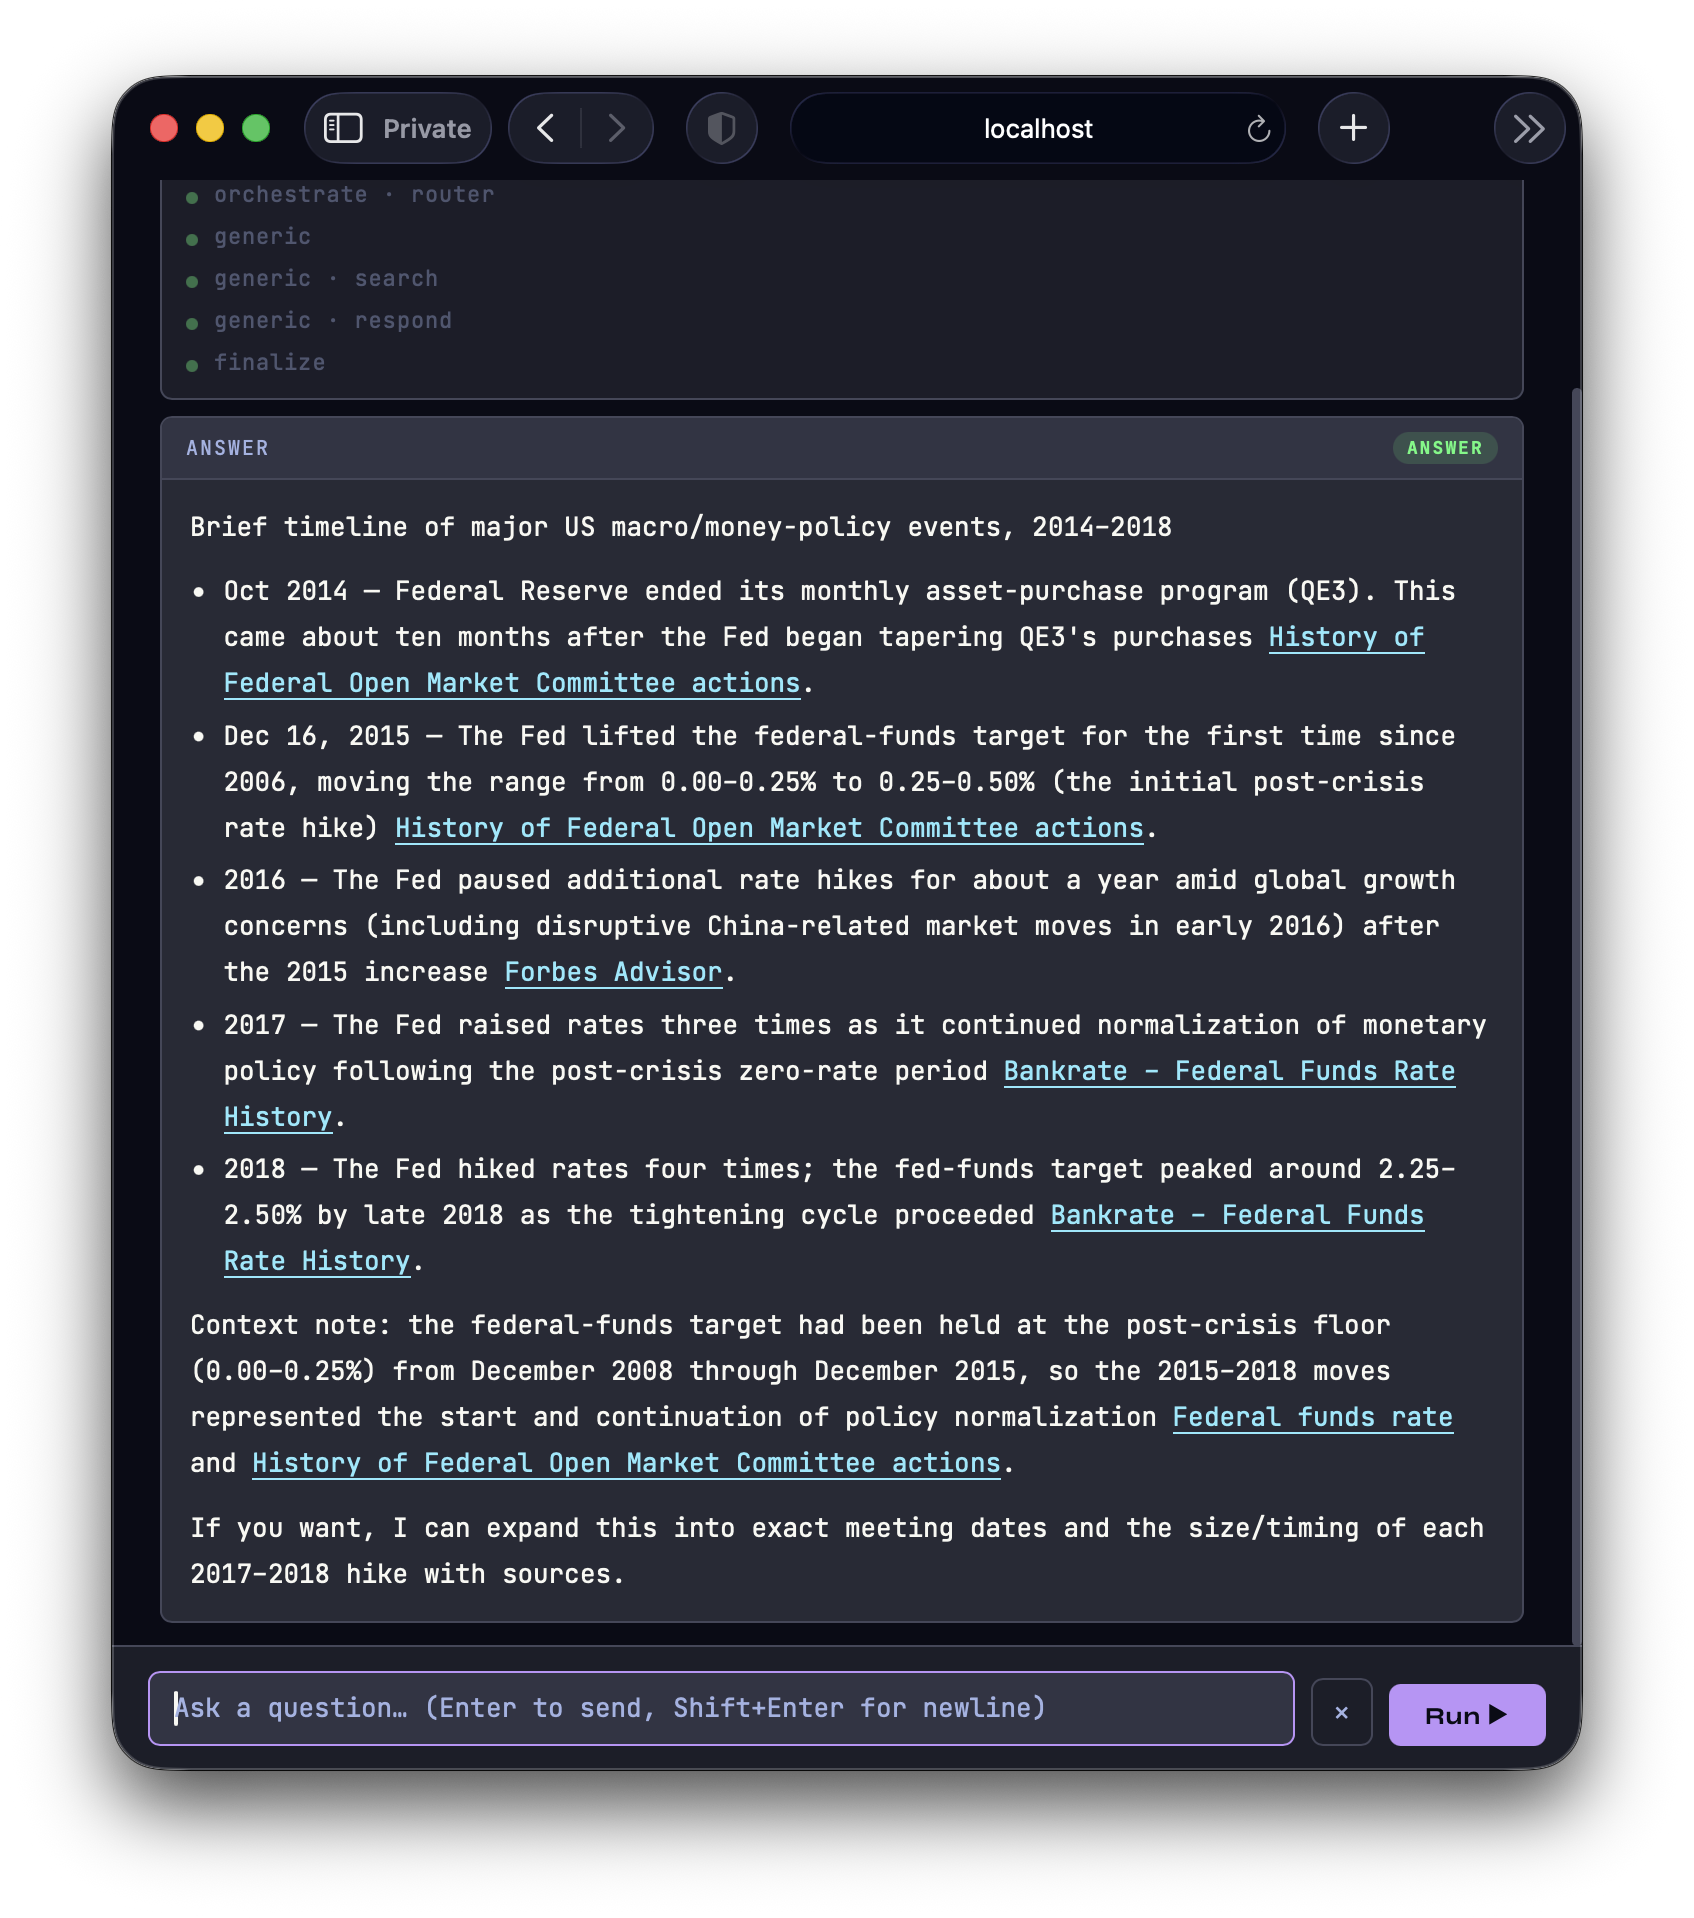
\includegraphics[width=0.4\textwidth]{graphics/ui-what-us-macroeconomic-events-rate-hikes,-policy-changes-occurred-between-2014-and-2018.png}
  \caption{UI Screenshot}
\end{wrapfigure}

The objective was to construct a chronological timeline of major US monetary policy shifts, specifically focusing on Federal Reserve actions (rate hikes and quantitative easing changes) between 2014 and 2018. The agent employed a temporal analysis strategy, prioritizing date keywords (\textit{2014}, \textit{2015}, \textit{2016}, \textit{2017}, \textit{2018}) and policy-specific terms (\textit{QE}, \textit{rate hike}, \textit{Federal Funds Rate}, \textit{tapering}).

\subsect{Step 1: Establishing the Starting Point (2014)}
The agent first queried for major shifts near the start date. The search results immediately highlighted the end of Quantitative Easing (QE3). Source [Wikipedia - OMF Committee actions] confirmed that the Federal Reserve ended its monthly asset purchases program (QE3) in \textbf{October 2014}, noting this followed a tapering process, thus marking a major policy shift from accommodative monetary policy.

\subsect{Step 2: Identifying the First Rate Hike (2015)}
The agent then focused on rate normalization post-crisis. Source [Wikipedia - OMF Committee actions] and [Forbes Advisor] consistently identified the critical event of \textbf{December 16, 2015}. The key action was raising the Federal Funds Rate for the first time since 2006, moving the target range from $0.00-0.25\%$ to $0.25-0.50\%$. This step established the start of "policy normalization."

\subsect{Step 3: Tracking Cyclical Changes and Pauses (2016-2018)}
The agent analyzed rate movements year-by-year.
\begin{itemize}
  \item \textbf{2016:} Source [Forbes Advisor] introduced the concept of a pause. The agent extracted that following the 2015 hike, the Fed paused additional rate hikes for approximately a year due to global growth concerns, specifically mentioning disruptive China-related market moves in early 2016.
  \item \textbf{2017:} Source [Bankrate] and [final\_answer.md] provided specific quantification. The agent determined that the Fed resumed hiking rates three times during 2017 as part of continued normalization efforts.
  \item \textbf{2018:} The trend accelerated. Source [Bankrate] confirmed that rates were raised four times in 2018, leading to a peak target rate near $2.25\%–2.50\%$ by the end of the year. This completed the tightening cycle phase analyzed.
\end{itemize}

\subsect{Step 4: Synthesis and Timeline Construction}
Finally, the agent synthesized these discrete points into a coherent narrative timeline, ensuring that the overall context (the shift from a multi-year zero-rate environment to aggressive normalization) was maintained. The agent used the contextual notes provided in $\text{\texttt{final\_answer.md}}$ to frame the entire period as "the start and continuation of policy normalization," providing a high-level summary ideal for the final answer structure.

\subsect{Conclusion}
The process successfully gathered both the specific dates/amounts (e.g., Dec 2015 rate hike) and the overarching narrative context (policy tightening cycle $2017 \rightarrow 2018$; pause in $2016$), resulting in a comprehensive, chronological report of major US macroeconomic policy shifts during the target window.
